\documentclass[a4paper,12pt]{article}

% 今回のTeXに使用するパッケージ
% 随時必要なパッケージを\usepackage{Package name}として宣言してください。
\usepackage{amsmath}  % 数式のためのパッケージ
\usepackage{amssymb}  % 数学記号 (\mathbbなど) のためのパッケージ
\usepackage{graphicx} % 画像挿入のためのパッケージ
\usepackage{booktabs} % 表のデザイン改善
\usepackage{hyperref} % ハイパーリンクのためのパッケージ

\title{LaTeX演習ファイル}
\author{あなたの名前}
\date{\today}

\begin{document}

\maketitle

\tableofcontents

\newpage

\section{イントロダクション}

このTexファイルに書かれている内容は、学部3年生向けにLaTeXの基本的な要素を説明することを目的としています。
LaTeXを使うことで、論文やレポートの作成が容易になります。演習も兼ねて記述の練習してみましょう。

\section{数式の種類と違い}

LaTeXでは、数式を表現するためにいくつかの方法が提供されています。以下では、それぞれの数式の違いを説明します。

\subsection{インライン数式}

インライン数式は、通常のテキストの中に組み込まれる小さな数式です。例えば、以下のように数式が文章中に表示されます。

中学校で習う比例の式は、$y=ax$($y$は比例定数)で表すことができます。また、\(y = x^n (n \in \mathbb{N})\)の微分は、
\begin{math}
    y' = nx^{n-1}
\end{math}
で求まります。
\subsection{ディスプレイ数式}

ディスプレイ数式は、独立した行として中央に配置される数式です。通常、複雑な数式や強調したい数式に使用されます。この形式では、数式が中央に配置され、大きめのサイズで表示されます。
例を以下に示します。
$$ x = a$$ から \[x = b \]までの関数$$f(x)$$の定積分は
\begin{displaymath}
    \int_a^b f(x) dx = F(b) - F(a)
\end{displaymath}
で定義される。


\subsection{番号つきディスプレイ数式}
中央に寄せつつ数式に番号をつけたい場合、番号つきディスプレイ数式を使用しましょう。以下に例を示します。
$f(x)$の不定積分は以下で定義される。ただし、$C$は積分定数である。
\begin{equation}
    \int^{b}_{a} f(x) dx = F(x) + C
\end{equation}
一方、$x = a$から$x=b$までの関数$f(x)$の定積分は、以下で定義される。
\begin{equation}
    \int_a^b f(x) dx = F(b) - F(a)
\end{equation}
このとき積分定数が消える理由は以下が理由である。
\begin{eqnarray}
    \int_a^b f(x) dx &=& \left[F(x) + C\right]_a^b  \\
    &=& \left(F(b) + C\right) - \left(F(a) + C\right) \\
    &=& F(b) - F(a)
\end{eqnarray}


\section{箇条書き}

LaTeXでは、箇条書きや番号付きリストも簡単に作成できます。

\subsection{箇条書きの例}
\begin{itemize}
    \item 最初の項目
    \item 2番目の項目
    \item 3番目の項目
\end{itemize}

\subsection{番号付きリストの例}
\begin{enumerate}
    \item 1つ目
    \item 2つ目
    \item 3つ目
\end{enumerate}

\section{図の挿入}

次に、画像を挿入する方法を説明します。画像はJPEG, PNGなどの形式に対応しています。ただし、pLaTeXの場合、pngなどではエラーが出る可能性があります。
そのため、eps形式を使用することを推奨します。

\begin{figure}[h]
    \centering
    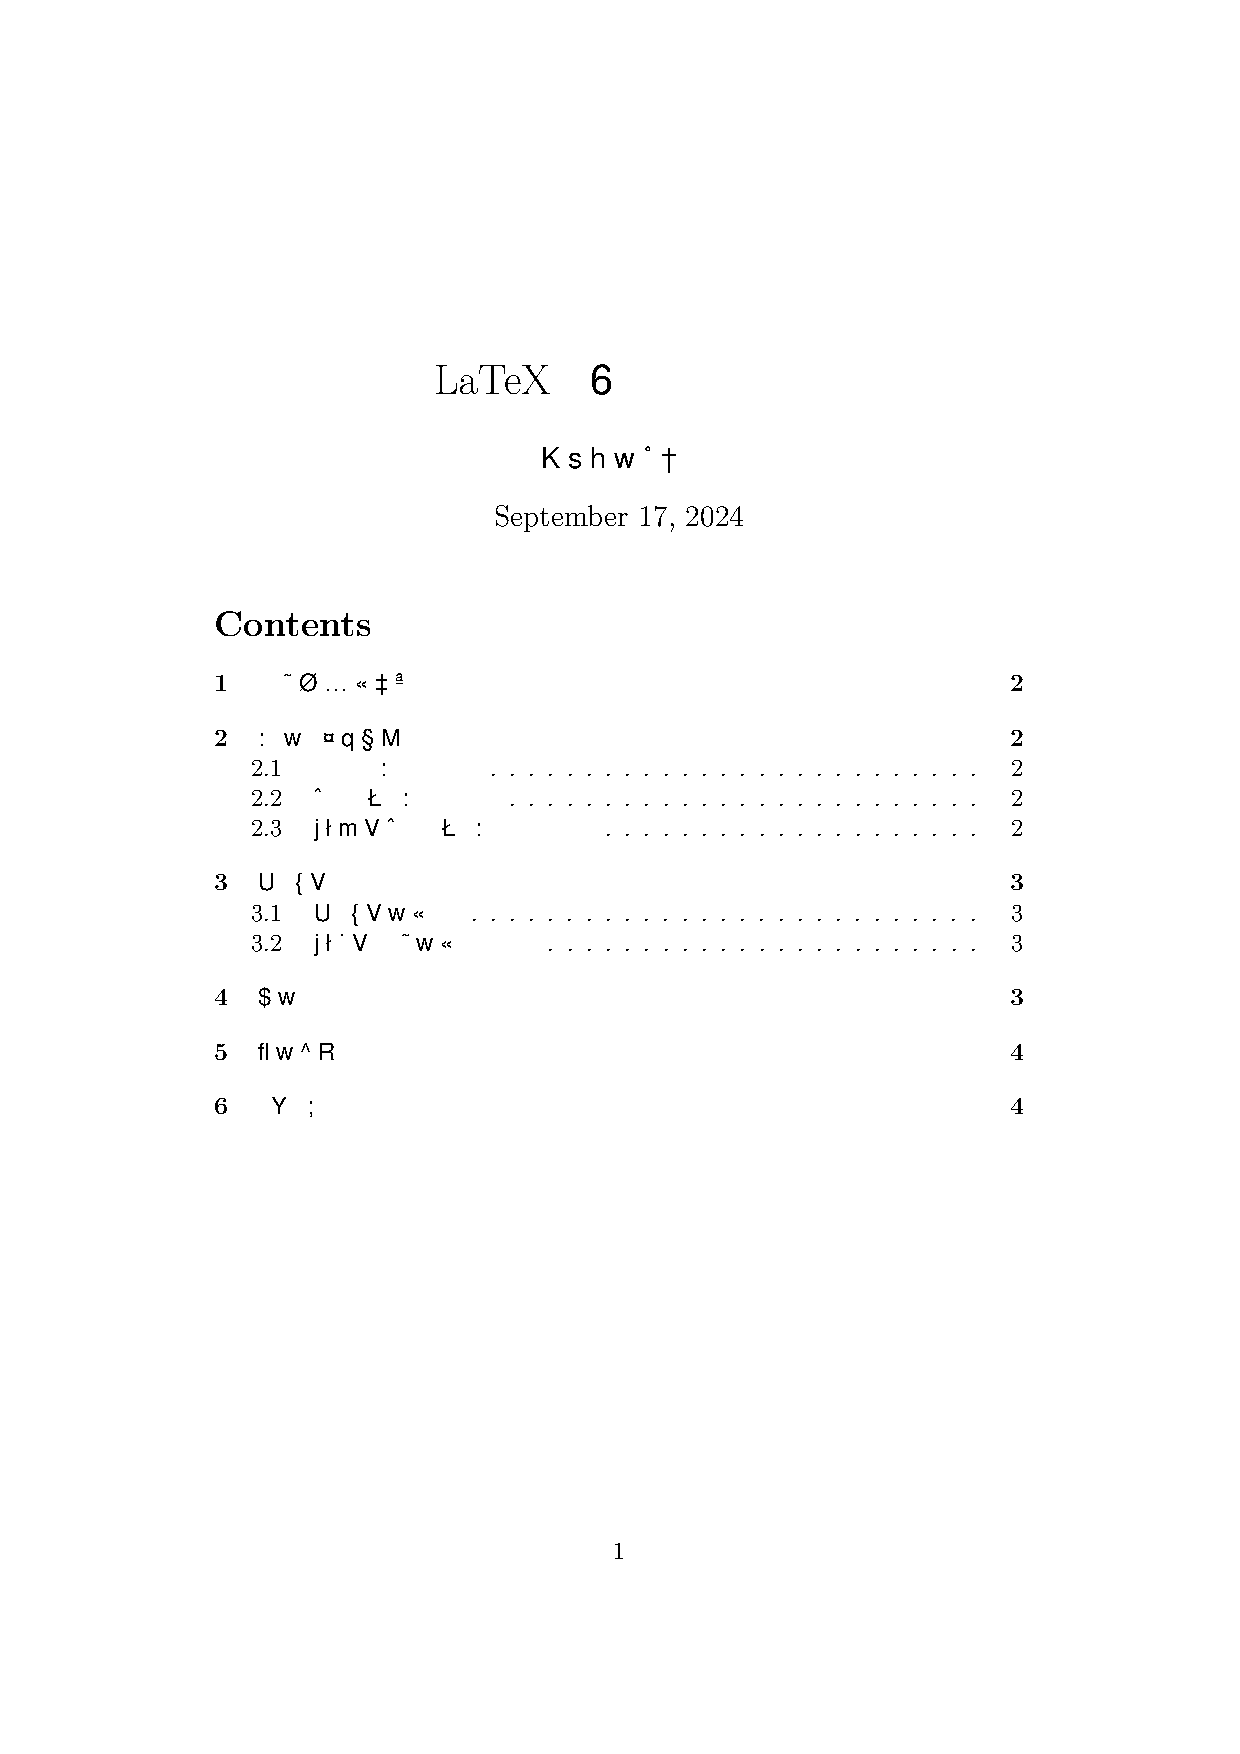
\includegraphics[width=4cm, height=4cm]{img/sample.eps2}
    \caption{サンプル画像のキャプション}
    \label{fig:sample}
\end{figure}

図\ref{fig:sample}は、LaTeXで画像を挿入した例です。

\section{表の作成}

LaTeXでは、表を簡単に作成することができます。次にその例を示します。

\begin{table}[h]
    \centering
    \begin{tabular}{lcc}
        \toprule
        項目 & 値1 & 値2 \\
        \midrule
        A & 100 & 200 \\
        B & 300 & 400 \\
        C & 500 & 600 \\
        \bottomrule
    \end{tabular}
    \caption{サンプル表}
    \label{tab:sample}
\end{table}

表\ref{tab:sample}は、項目ごとのデータを示しています。

\section{文献引用}
論文を書く上で参照した論文や書籍、サイトなどは必ず引用する必要があります。
引用方法は、指定があるパターンが多いため確認を忘れないようにしましょう。また、初回ビルド時は、引用箇所が[?]となってしまうため、必ず2回以上行ってください。
引用方法の例を以下に示します。
樋口らは、eBPFを用いたリアルタイム防御システムを考案した\cite{Higuchi2023}。

\begin{thebibliography}{1}
\bibitem{Higuchi2023}K. Higuchi and R. Kobayashi, "Real-Time Defense System using eBPF for Machine Learning-Based Ransomware Detection Method," 2023 Eleventh International Symposium on Computing and Networking Workshops (CANDARW), 2023, pp. 213-219, doi: 10.1109/CANDARW60564.2023.00043. 
\end{thebibliography}

\end{document}

